\chapter[Lessons learnt using a pre-trained AI model]
{Lessons learnt using a pre-trained AI model\pubfootnote{Graetsch:2020ase-industry}}
\label{ch:ase2020-industry}
\graphicspath{{mainmatter/publications/figures/ase-industry2020/}}

\glsresetall
\begin{abstract}
Pre-trained \glsac{ai} models are increasingly available as \glsacpl{api} and tool-kits to software engineers, making complex \glsac{ai}-enabled functionality available via standard and well-understood methods. However, reusing such models comes with risks relating to the lack of transparency of the model and training data bias, making it difficult to confidently employ the toolkit in a new situation.  Vendors are responding and proposing artefacts such as model cards and datasheets to make models and their training more transparent.  But is this enough?  As part of an investigation into determining if a cloud-based \glslong{iws} was ready for production use, we processed developer questions on \glslong{so} using a published pre-trained classifier that was specifically tuned for the software engineering domain. In this paper, we present lessons learnt in this automation effort. We find the results were unexpected and led us to delve into model and training data---an option available to us because the information was available for research.  We found that had a model card and datasheet been prepared, we could have identified risks to our study earlier on. However, model cards and datasheets specifications are not yet mature enough and additional tools and processes are still required to confirm a decision whether a model can be reused with confidence.
\end{abstract}
\glsresetall

\section{Introduction}
Pre-trained \glsac{ai} models are increasingly available to software engineers either directly or wrapped into web-based components and toolkits.\footnote{For example, Google's Cloud \glsac{ai} or Microsoft Azure's Cognitive Services.} The grand promise is the rapid creation of \glsac{ai}-infused functionality into end-applications as developers can simply reuse models instead of training them from scratch, as training is laborious and resource-intensive~\citep{RamanAnandHoder2015}. Vendors do provide usage guidelines, component documentation, code examples and a compelling marketing narrative, although the limitations and risks are not as well-presented in  official documentation~\citep{Cummaudo:2019icsme,Cummaudo:2020icse}. 
In practice, developers and technical architects study issue trackers and online forums such as \gls{so} to assess and inform their decisions. This is also complemented by multiple studies that highlight the value and insights to be gained from these online forums~\citep{Abdalkareem2017WhatOverflow,Storey2014}.

This paper is the result of an investigation into determining if cloud-based \glspl{iws} are ready for a specific industry use case. Inspired by the possibility of finding insight from content in the online forums, we wanted to analyse the questions posed and issues raised---in particular on \gls{so}---that relate to that relate to  \glspl{iws} that provide computer vision (i.e., \glslongpl{cvs} or \glsacpl{cvs}).  Although a manual analysis is possible, we wanted to automate this process using natural language processing techniques, which was motivated by (i) the gain from automation---specifically having a repeatable process that can be tuned to focus on different aspects---and, more importantly, (ii) to learn about potential issues with these pre-trained models as we use one of these services to turn on themselves.

In our analysis, beyond the direct summative aspects, we focused on emotions within the content posed on the online forums. This was motivated by work done by~\citet{wrobel2013}, who suggested that frustration and anger were amongst the emotions that posed the highest risk to developer productivity. Our goal was to determine if negative emotions such as anger or frustration are the predominant theme within questions on these forums: the natural expectation is that developers would not pose questions unless they needed support and help. Similarly, we would expect the tone of responses to be neutral and hopefully supportive. Our focus, however, remains on the questions posed.

Our findings, elaborated further in  \cref{ase2020-industry:SubSection:Findings}, were surprising. While the pre-trained model we selected was trained specifically on \gls{so} and tuned for emotions~\citep{novielli2018,calefato2017}, our results show that 14\% issues can be considered in the category of \textit{Love} or \textit{Joy}, and a surprising small amount (5\%) are in the category of \textit{Anger} (or frustration). A closer examination using multiple human reviewers showed an even more interesting insight: the reviewers did not agree with the automated machine classification, and worse, the reviewers did not agree with each other, suggesting that training machines with a consistent set of labels is a non-trivial exercise.  Finally, we reflected whether the pre-trained classifier could be better documented.  We found vendors are recognising these challenges and are offering solutions to better document their models~\citep{Mitchell:2018in, Gebru:2018wh}. However, when we looked into the information captured by these solutions, we found their specification to be very broad and additional guidance for completion is required to help evaluate risks faced in an industry context (discussed in \cref{ase2020-industry:subsec:ModelCards}).

\section{Case Study}\label{ase2020-industry:sec:study}
In this section, we discuss the case study which inspired the initial objective of investigating if cloud-based \glspl{iws} were ready for use in an industrial context. To permit replication, the raw results produced from this case study are made available online at \url{https://bit.ly/36DIARI}.

\subsection{Scope} 
To align with our use case, we narrowed our focus to cloud-based \glspl{cvs}. Recent research has identified growth in questions on \gls{so} relating to such services, giving us confidence that we would have a rich data set~\citep{Cummaudo:2020icse}.  We decided to explore emotions expressed by developers through the questions they pose on \gls{so} to identify whether developers are surprised, angry, frustrated, or overall positive? Previous works into developer questions show that despite the technical nature, their communications on \gls{so} do exhibit emotions~\citep{Novielli:2015vda, calefato2017}.  Although we could have read these posts manually, for consistency, repeatability, and efficiency, we chose to automate this process by utilising an emotion aware text classification system trained specifically on \gls{so} \citep{novielli2018}. Our expectation was that we would gain some insight into the questions through the emotions, and we hypothesised that we would see a high proportion of surprise (i.e., the \glsac{api} does not work as expected) and anger (frustration due to mismatched expectations).

\subsection{Method}
\label{ase2020-industry:sec:study:method}
We selected a published peer-reviewed emotion model as the text classifier. This classifier is included in the EMTk llkit and has been specifically trained for emotional text classification in the software engineering domain~\citep{calefato2017}. The EMTk toolkit is available with a fully labelled training dataset~\citep{novielli2018}, permitting reuse and analysis of internals.  The classifier is based on \citeauthor{shaver1987}'s emotional hierarchy model~\citep{shaver1987} and performs binary classifications against text data provided in input files and an input parameter designating the emotion to be classified---one of \textit{Love}, \textit{Joy}, \textit{Surprise}, \textit{Fear}, \textit{Sadness} or \textit{Anger}. As input for the classifier, we used a dataset of the 1,425 \gls{so} questions restricted to intelligent \glspl{cvs} available in~\citep{Cummaudo:2020icse} and we ran the classifier with the same input dataset for each of the six emotions.
To cross-check classified output, we manually annotated a random sample of 25 questions.  Each of these 25 posts were assigned to three raters who carried out the following three steps: (i) identify the presence of emotion(s); (ii) if emotion(s) exists, classify the emotion(s) under one of the six basic emotions as per the Shaver framework. After collating each rater's results, we calculated a Fleiss' Kappa~\citep{Fleiss:1971ff} as a measure of inter-rater agreement per emotion for each of the three human raters (manual rating). We then used the results from the classifier as a `fourth' \textit{automated} rater, comparing the results with the manual rating by calculating the agreement for each emotion and calculated the observed percentage of agreement and Fleiss' Kappa for further inter-rater agreement analysis.

\subsection{Results} \label{ase2020-industry:SubSection:Findings}

Of the 1,425 \gls{so} questions, the classifier did not classify any emotion to 622 posts (labelled \textit{No Emotion}). The remaining posts were classified: 224 posts as \textit{Fear}, 223 as \textit{Surprise}, 70 as \textit{Sadness}, 103 as \textit{Love}, 100 as \textit{Joy}, and 76 as \textit{Anger}. Some posts classified against two or more emotions, and as a result, the total proportions do not add up to exactly 100\%. 
Results from our inter-rater analysis are reported in \cref{ase2020-industry:table:2}.

\begin{table}[t]
\caption{Results from Inter-Rater Agreements.}
\label{ase2020-industry:table:2}
\centering
\begin{tabular}{l|cc}
\toprule
\textbf{Emotion}&
\textbf{Three Raters}&
\textbf{Three Raters + Classifier}\\
\midrule
Anger&0.256&0.145\\
Fear&-0.014&-0.075\\
Joy&0.306&0.132\\
Love&1.000&-0.031\\
Sadness&-0.071&-0.053\\
Surprise&-0.056&-0.091\\
No Emotion&0.265&0.139\\
\bottomrule
\end{tabular}
\end{table}

Guidelines of indicative strengths of agreement are provided by~\citet{Landis:1977kv}, where: $\kappa \leq 0$ indicates \textit{poor} agreement; $0 < \kappa \leq 0.2$ indicates \textit{slight} agreement; $0.2 < \kappa \leq 0.4$ indicates \textit{fair} agreement; $0.4 < \kappa \leq 0.6$ indicates \textit{moderate} agreement; $0.6 < \kappa \leq 0.8$ indicates \textit{substantial} agreement. When using the classifier's output as a fourth `rater', there was slight agreement on \textit{Anger}, \textit{Joy}, and \textit{No Emotion}. Between the three human raters, those same emotions were rated with fair agreement.  Agreement for \textit{Love} was unanimous amongst the three human raters, finding zero instances of \textit{Love} across the sample (thus resulting in a kappa value of 1.00). Inter-rater agreement was poor for the \textit{Fear}, \textit{Sadness}, and \textit{Surprise}.

\section{Findings and Discussion}
In this section, we reflect on our results with respect to limitations in the classifier and investigation of the peer-reviewed and published dataset used to train the classifier. Given the weak results, we also investigate whether model cards~\citep{Mitchell:2018in} and/or datasheets~\citep{Gebru:2018wh} could have provided a more effective approach to informing the viability and limits of the pre-trained model.

\subsection{Limitations of the Text Classifier}
The classifier did not assign any emotion to 43\% posts.  This result corroborates the findings by~\citeauthor{murgia2014}, who identified via a manual process \textit{No Emotion} as the most prevalent classification~\citep{murgia2014}. For illustration, we provide a set of examples in \cref{ase2020-industry:table:SomeAgreement}. (The numbers in the raters column indicate the count of raters who assigned this label.) In the first example, each human rater assigned a different emotion to the same question, despite the classifier classifying it with \textit{No Emotion}. The second example also highlights discrepancy between raters (two raters agree on \textit{Joy}) but the classifier classified it as \textit{Love}. Lastly, the third example highlights one example of consistency between all three raters and the classifier.

\begin{landscape}
\begin{table}[p]
\caption[Sample questions comparing EmoTxt to manual classification]{Sample questions comparing EmoTxt to manual classification. Questions located at: https://stackoverflow.com/q/[ID].}
\label{ase-industry2020:table:SomeAgreement}
\centering
\begin{tabular}{p{0.1\linewidth}p{0.44\linewidth} p{0.09\linewidth} p{0.11\linewidth}}
\toprule
\textbf{Question ID}&
\textbf{Quote}&
\textbf{EmoTxt}&
\textbf{Raters}\\
\midrule
54521080&
\textit{``I am aware that it is better to use AWS Rekognition for this. However, it does not seem to work well when I tried it out with the images I have (which are sort of like small containers with labels on them). The text comes out misspelled and fragmented.  I am new to ML and Sagemaker ... Is it possible to to do it with Sagemaker? I would appreciate it if someone pointed me in the right direction.''}& 
No Emotion &
Fear (1) \newline Sadness (1) \newline {Surprise} (1)\\
52446033
&\textit{``I am using the Google Cloud Vision \glsac{api} to search similar images (web detection) and it works pretty well. Google detects full matching images and partial matching images (cropped versions).  I am looking for a way to detect more different versions. For example, when I look for a logo, I would like to detect large, small, square, rectangular versions of this logo. For now, I detect images that match exactly the one I upload and cropped versions.  Do you know if this is possible and how can I do that?''}& 
{Love} &
{Joy} (2) \newline {No Emotion} (1)\\
54677464&
\textit{``I have implemented a QR scanner(QRScanner class) using Google Vision \glsac{api}. Once a value is detected it is passed to another activity(Info class) using Intents. The problem is that once a QR code is scanned the Info class gets opened several times.I want to limit the QRScanner class to get only one QR value and Info classed to be opened only once.  Currently once a QR is detected the Info class gets called several times. I want the QRScanner to get only one value and Info class to get called only once.''}&
{No Emotion} &
{No Emotion} (3)\\
\bottomrule
\end{tabular}
\end{table}
\end{landscape}
\subsection{Peering into the Training Dataset}
We investigated the training dataset and related research documentation to see if that would give us further insights.  We found two areas warranting further exploration---training data balance and training data annotation. 

\subsubsection{Data imbalance}
 We found that the purpose of the training dataset was actually to train two classifiers---a sentiment classifier and an emotional classifier.  Each post in the training dataset was labelled with zero, one or more emotions. In addition, emotions were grouped, i.e., the positive emotions of \textit{Joy} and \textit{Love} were grouped into positive sentiment while \textit{Sadness}, \textit{Anger} and \textit{Fear} were grouped into negative sentiment. \textit{Surprise} was assigned either positive or negative sentiment, depending on context~\citep{novielli2018, calefato2018}.  \cref{ase2020-industry:fig:data-imbalance-training} shows the distribution of emotion labels across 4,800 posts in the training dataset; \textit{No Emotion} is removed to emphasise emotion-only results. (Total count: 1959.)

\begin{figure}
    \centering
    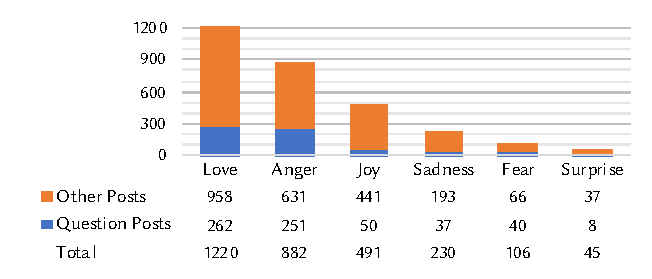
\includegraphics[width=.8\linewidth]{data-imbalance.pdf}
    \caption [Emotion classifier training data imbalance]{The emotion classifier training dataset distribution is largely skewed toward \textit{Love}, resulting in data imbalance. (\textit{No Emotion} labels were removed from this graph.)}
    \label{ase2020-industry:fig:data-imbalance-training}
    % \vspace{-.5cm}
\end{figure} 

Class imbalance and its impact on classifier models is a known problem in machine learning~\citep{Lopez2014, Weiss2004}, where  one class (known as the majority, positive class) significantly outnumbers the other class (known as the minority, negative class).  The impact of class imbalance on classification models results in minority classes with lower precision and lower recall than the majority class, since the classifier does not generate rules for the minority class.  One set of relevant techniques for addressing class imbalance is data sampling; including undersampling or subsampling, oversampling and hybrid approaches~\citep{Lopez2014}.
Whilst the training dataset seems balanced for the purpose of sentiment analysis, there is a lack of balance across individual emotions.  The predominant emotion in the training dataset was \textit{No Emotion} at 40.8\% of total posts. The most dominant emotions were \textit{Love} and \textit{Anger} at 25\% and 18\% respectively.  Less than 1\% of posts were labelled with \textit{Surprise}.  This means that the number of posts falling into some of the categories, for example, \textit{Surprise} and \textit{Fear} (i.e., 45 and 106 posts, respectively) is very low for training purposes. 

Further, the training dataset was spread across different types of \gls{so} posts (i.e., questions posts, answer posts, question comments, answer comments) to capture the different emotional language, however our study was interested in classifying \gls{so} question posts only. Of the training dataset's 4,800 posts, only 1,044 were question posts and within that subset of posts, the distribution of emotions was more polarised than in the overall 4,800 posts. \textit{Love} and \textit{Anger} are the most predominant emotions in the training dataset, however \textit{Anger} has a higher proportion (24\%) in question posts, as opposed to only 18.4\% in the overall dataset. 

In summary, the training dataset was not balanced within each emotion category and some emotions had very low sample numbers, as emphasised in the skew in \cref{ase2020-industry:fig:data-imbalance-training}.  Proportions of training data examples per question per emotion was very low for \textit{Joy}, \textit{Surprise}, \textit{Sadness} and \textit{Fear}.
To address this imbalance and achieve better performance, training data could be enhanced to include additional samples or to use an oversampling approach.  A recent study into class-balancing approaches in the context of defect prediction models found that class rebalancing does lead to a shift in the learned concepts~\citep{Turhan2012OnModels}.

\subsubsection{Emotion labeling bias}\label{ase2020-industry:SubSubSection:EmotionLabelingBias}
In software engineering, hierarchical categorical emotional frameworks including those featured in \citet{Parrott2001}, \citet{Ekman1978} and \citet{shaver1987} have been assessed by researchers and pragmatically selected as the basis for training emotional classifiers.  The chosen emotion framework is then used as the taxonomy truth labels for classifier training datasets.  Data for labeling is sourced from systems such as \gls{so} and JIRA ~\citep{murgia2014, ortu2016, gachechiladze2017, novielli2018}.  In the software engineering domain, truth labeling of emotions has to date been done manually~\citep{murgia2014, novielli2018, gachechiladze2017}.  Emotion annotation involves at least a pair of annotators~\citep{Ghazi2010HierarchicalTexts, Aman2007IdentifyingText}. For the EMTk training dataset, annotation was performed manually by a team of 12 coders, divided into four groups of three with a computer science background~\citep{calefato2017, novielli2018}.  Manual annotation challenges when coding emotions can be encountered due to different levels of semantic ambiguity within emotions and how humans express emotions in text~\citep{Hasan2014UsingMessages}. In the absence of an objective emotional truth, researchers' consistency is taken as a measure of correctness---i.e., multiple annotators that agree~\citep{murgia2014}.  A measure of inter-rater agreement is Cohen's Kappa~\citep{Cohen:1960tf} (for two raters) or  Fleiss' Kappa~\citep{Fleiss:1971ff} for more raters.  For the training data set, inter-rater agreement ranged from  $\kappa=0.30$ (fair) for \textit{Joy} to $\kappa=0.66$ (substantial) for \textit{Love}.  The researchers specifically trained dataset coders for consistency. The challenge of this approach with a subject such as emotions is the opportunity for bias.  In contrast, in other studies, researchers specifically attempted to reduce the opportunity for biases by including raters with different nationalities, skills, cultural backgrounds, by increasing the number of raters~\citep{ortu2016} and opting against consistency training~\citep{Alm2005EmotionsText}.  As such, the approach taken to achieve consistency and makeup of label coders is important information for downstream consumers of an \glsac{ai} model.

\subsubsection{Emotion labeling and classification granularity}
Training data annotation was performed on \gls{so} posts---which included questions, answers, and comments to questions and answers.
Emotion annotation can be performed at different levels of granularity---word level~\citep{StrapparavaWordNet-Affect:WordNet}, spans of words in a sentence~\citep{Aman2007IdentifyingText}, sentence level or larger.  While a word level or keyword approach is considered too granular (as it does not capture the emotional context sufficiently), there is a risk of emotion progression during narratives and also within sentences~\citep{Aman2007IdentifyingText, murgia2014}.  Our \gls{cvs} dataset consisted of questions only as we were seeking to assess developer emotion expressed at the time of raising the question.  Question posts are typically longer than comments and may contain multiple emotions expressed at different levels of intensity that are interpreted differently by different readers.  For example, in the first question in \cref{ase2020-industry:table:SomeAgreement} the first sentence does not carry any emotion while in the second part the reader expressed \textit{Surprise} that the \glsac{api} does not work in all cases (\textit{Surprise}/\textit{Sadness}) and their lack of experience (\textit{Fear}), and appreciation (possibly \textit{Love}).   

\subsection{New tools: Model Cards and Datasheets}\label{ase2020-industry:subsec:ModelCards}
Model cards are emerging tools proposed by Google to communicate performance characteristics of pre-trained models~\citep{Mitchell:2018in}.  Google have recently published sample model cards relating to their Cloud Vision \glsac{api}.\footnoteurl{https://modelcards.withgoogle.com/model-reports}{25 May 2020}  Microsoft have focused on a standardised process of dataset documentation through datasheets to encourage transparency and accountability by documenting the motivation, composition, collection process and intended uses of data~\citep{Gebru:2018wh}.  IBM have proposed a FactSheet concept combining model and data information~\citep{Arnold2019FactSheets:Conformity}.  These tools are being adopted by organisations and researchers;  for example, Open \glsac{ai} have published a basic model card of their generative language model and Google provided a sample model card for their Toxicity analyser~\citep{Mitchell:2018in}.  Model cards are also being considered for high stakes environments such as clinical decision making~ \citep{Sendak2020PresentingLabels}, where they facilitate overarching governance regimes on how and when models can be used.
For our case study, a combination of Model Card for the classifier and datasheet for training data could have provided a valuable, easy to digest first step to support an evaluation of the classifier for our context.  However, the current specification of datasheet contents is very broad and lacks detailed directions for those completing the information.  Had all the required information been provided to sufficient detail, including a highlight of the importance of consistency training, we could have better assessed whether an emotion assessment was appropriate.  However, we would still have had to complete the study---but with rater consistency training and a better appreciation of the limits of the classifier. 

\subsection{Threats to validity} 
 We sampled only 25 posts for inter-rater reliability and it remains a limitation of our analysis.  Although, only 25 posts were sampled for inter-rater reliability, the first author reviewed an additional 500 posts and the inconsistency observed from the 25 posts maps to the broader analysis.

%\subsection{Further research opportunities}
%To do---

\section{Conclusion}\label{ase2020-industry:sec:conclusion}
We started the journey presented in this work with an idea to use existing \glsac{ai} techniques to \textit{automatically} investigate what other developers think of cloud intelligent services. This translated into our attempt to use a  pre-trained model that learnt from posts provided by software engineers on \gls{so}.

Developers learn, improve and deepen their skills from documentation, formal or self-paced education, experience, and sharing their knowledge. Good documentation often forms the foundation that enables learning and also to create educational aids. In this work, we presented an observation case study that highlights a set of gaps in how a peer-reviewed model, published in the field of software engineering, lacks information about the limitations both within the documentation, as well as the articles published. To resolve these gaps, we investigated if new solutions that are being proposed such as model cards would have helped us. Model cards and datasheets will be a necessary and helpful first step, but as such we found their specification to be insufficient and additional guidance is required for those completing the cards and datasheets. Although we study only one pre-trained model in depth, our analysis shows that there are gaps in proposed solutions that can be addressed and our future work will focus on investigating other models and \glspl{iws} to develop a more detailed documentation approach, specifically those that are being aimed for software engineering. 